\documentclass[a4paper,12pt]{article}
\usepackage{amsmath}
\usepackage{hyperref}
\usepackage{listings}
\usepackage{xcolor}
\usepackage{graphicx}
\usepackage{tocloft} % For customizing table of contents
\usepackage{titlesec} % For section formatting
\usepackage{geometry} % For margin control
\usepackage{fancyhdr} % For header and footer
\usepackage{enumitem} % For list customization
\usepackage{float}

\geometry{
    a4paper,
    top=2.5cm,
    bottom=2.5cm,
    left=2.5cm,
    right=2.5cm
}

\lstdefinelanguage{octave}{
  keywords={break,case,catch,continue,else,elseif,end,for,function,
    global,if,otherwise,persistent,return,switch,try,while},
  keywordstyle=\color{blue},
  identifierstyle=\color{black},
  sensitive=false,
  comment=[l]{\%},
  commentstyle=\color{codegreen},
  stringstyle=\color{magenta},
  morestring=[m]'
}

\setlist[itemize]{topsep=0pt,itemsep=2pt,partopsep=0pt,parsep=0pt}
\setlist[enumerate]{topsep=0pt,itemsep=2pt,partopsep=0pt,parsep=0pt}

% Custom bullet points
\renewcommand{\labelitemi}{$\bullet$}
\renewcommand{\labelitemii}{$\circ$}
\renewcommand{\labelitemiii}{$\diamond$}
\renewcommand{\labelitemiv}{$\cdot$}

\pagestyle{fancy}
\fancyhf{}
\fancyhead[L]{\slshape\nouppercase{\leftmark}}
\fancyhead[R]{\thepage}
\renewcommand{\headrulewidth}{0.4pt}

% Customize section formatting
\titleformat{\section}
    {\normalfont\Large\bfseries}{\thesection}{1em}{}
\titleformat{\subsection}
    {\normalfont\large\bfseries}{\thesubsection}{1em}{}

% Customize TOC appearance
\renewcommand{\cftsecfont}{\bfseries}
\renewcommand{\cftsecpagefont}{\bfseries}
\setlength{\cftbeforesecskip}{10pt}
\setlength{\cftbeforesubsecskip}{5pt}

% Custom colors for listings
\definecolor{codegreen}{rgb}{0,0.6,0}
\definecolor{codegray}{rgb}{0.5,0.5,0.5}
\definecolor{codepurple}{rgb}{0.58,0,0.82}
\definecolor{backcolour}{rgb}{0.95,0.95,0.92}

% Listing style configuration
\lstdefinestyle{mystyle}{
    backgroundcolor=\color{backcolour},   
    commentstyle=\color{codegreen},
    keywordstyle=\color{magenta},
    numberstyle=\tiny\color{codegray},
    stringstyle=\color{codepurple},
    basicstyle=\ttfamily\footnotesize,
    breakatwhitespace=false,         
    breaklines=true,                 
    captionpos=b,                    
    keepspaces=true,                 
    numbers=left,                    
    numbersep=5pt,                  
    showspaces=false,                
    showstringspaces=false,
    showtabs=false,                  
    tabsize=2
}
\lstset{style=mystyle}



\title{Scientific Calculator Program in Octave}
\author{S.A.Abdulla - 22000021}
\date{21 January 2025}

\begin{document}
\maketitle

\newpage
\tableofcontents
\newpage

\newpage
\section*{Introduction}
\addcontentsline{toc}{section}{Introduction}

This scientific calculator program developed in Octave is designed to offer a wide range of mathematical functionalities, making it suitable for both basic and advanced calculations. The calculator allows users to perform standard arithmetic operations like addition, subtraction, multiplication, and division. However, its true strength lies in its ability to handle scientific and complex mathematical equations with precision and ease.

\section*{Prerequisites}
\addcontentsline{toc}{section}{Prerequisites}

\begin{itemize}
    \item \textbf{Software Required:}
    \begin{itemize}
        \item GNU Octave version 9.0 or higher.
    \end{itemize}
\end{itemize}

\section*{Installation Instructions}
\addcontentsline{toc}{section}{Installation Instructions}

\begin{itemize}
    \item \textbf{Operating System:} The program works on Windows, macOS, and Linux.
    \item \textbf{Octave Version:} GNU Octave 5.0 or higher is required for full compatibility.
    \item \textbf{RAM and Processor:} The calculator is lightweight and runs efficiently on most modern systems with minimal resource requirements.
\end{itemize}

\section*{How to Run the Calculator}
\addcontentsline{toc}{section}{How to Run the Calculator}

\begin{enumerate}
    \item Open Octave.
    \item Download or copy the \texttt{calculator.m} file to a directory on your system.
    \item In the Octave command window, navigate to the directory where \texttt{calculator.m} is saved using the \texttt{cd} command:
    \begin{lstlisting}[language=bash]
    cd('path/to/directory')
    \end{lstlisting}
    \item Run the calculator by typing:
    \begin{lstlisting}[language=octave]
    octave calculator.m
    \end{lstlisting}
\end{enumerate}

\section*{UI of calculator}
\addcontentsline{toc}{section}{UI of calculator}
\begin{figure}[H]
    \centering
    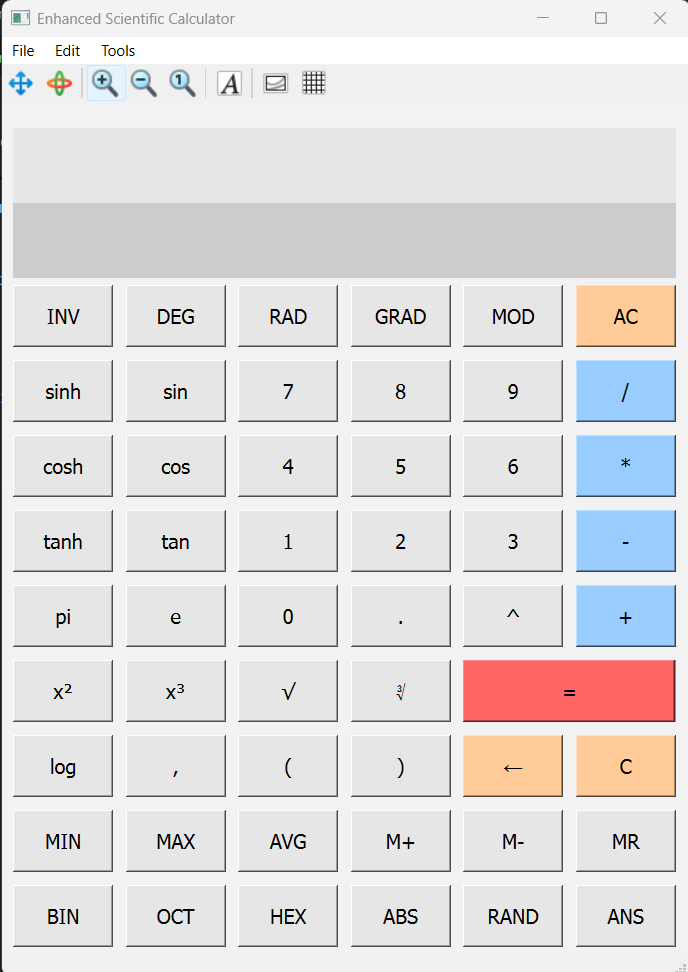
\includegraphics[width=\textwidth]{cal.png}
    \caption{Overview of the Scientific Calculator Interface} 
    \label{fig:calculator}
\end{figure}
\newpage

\section{Usage Instructions}a
\addcontentsline{toc}{section}{Usage Instructions}

Once the program starts, the calculator interface will be displayed, mimicking a physical scientific calculator. The user interacts with the calculator by selecting buttons for operations, entering numbers, and constructing equations. The interface dynamically displays the entered equation and results separately, ensuring clarity.

\subsection{Basic Usage}

The calculator supports basic arithmetic operations such as:

\begin{itemize}
    \item \textbf{Addition (+)}: Press the \texttt{+} button after entering the first number, followed by the second number, to see the result.
    \item \textbf{Subtraction (-)}: Press the \texttt{-} button to subtract one number from another.
    \item \textbf{Multiplication (*)} and \textbf{Division (/)}: Use the \texttt{*} and \texttt{/} buttons respectively for these operations.
\end{itemize}

\subsection{Advanced Functionalities}

The calculator extends beyond basic arithmetic with a comprehensive set of scientific operations and features:

\begin{itemize}
    \item \textbf{Trigonometric and Hyperbolic Functions}: Calculate \texttt{sin}, \texttt{cos}, \texttt{tan}, and their hyperbolic counterparts (\texttt{sinh}, \texttt{cosh}, \texttt{tanh}) by pressing the corresponding buttons. Use angle mode buttons (\texttt{DEG}, \texttt{RAD}, \texttt{GRAD}) to toggle the input angle unit.
    \item \textbf{Powers and Roots}: Compute squares (\texttt{x²}), cubes (\texttt{x³}), square roots (\(\sqrt{}\)), and cube roots (\(\sqrt[3]{}\)) effortlessly.
    \item \textbf{Scientific Constants}: Use constants like \texttt{pi} and Euler's number (\texttt{e}) in your equations without manual input.
    \item \textbf{Logarithmic Functions}: The \texttt{log} button calculates the natural logarithm of a number, while other base-specific logs can be added to future versions.
    \item \textbf{Modulo Operation}: Use the \texttt{MOD} button for modulus calculations to determine remainders.
\end{itemize}

\subsection{Equation Input and Display}

The calculator allows users to construct complex equations with parentheses, ensuring the correct order of operations. For example:

\begin{enumerate}
    \item Enter the equation: \texttt{(5 + 3) * 2}.
    \item Press the \texttt{= (equals)} button to calculate the result.
    \item The entered equation is displayed clearly at the top of the interface, while the result is shown separately below.
\end{enumerate}

\subsection{Memory Functions}

The calculator includes memory functionality to store and manage values:

\begin{itemize}
    \item \textbf{M+}: Add the displayed result to memory.
    \item \textbf{M-}: Subtract the displayed result from memory.
    \item \textbf{MR (Memory Recall)}: Retrieve the stored value for use in calculations.
    \item \textbf{Clear Memory}: If the memory is empty or needs resetting, the calculator will display \texttt{Memory Empty}.
\end{itemize}

\subsection{Statistical Calculations}

For statistical data analysis, the calculator provides:

\begin{itemize}
    \item \textbf{MIN}: Calculate the minimum of a set of numbers.
    \item \textbf{MAX}: Determine the maximum value.
    \item \textbf{AVG}: Compute the average of a set of values.
\end{itemize}

\subsection{Number System Conversion}

The calculator supports conversions between number systems:

\begin{itemize}
    \item \texttt{BIN}, \texttt{OCT}, and \texttt{HEX} buttons convert values to binary, octal, and hexadecimal formats respectively.
\end{itemize}

\subsection*{Random Number Generation and Special Functions}

\begin{itemize}
    \item \texttt{RAND}: Generate random numbers.
    \item \texttt{ABS}: Calculate the absolute value of a number.
    \item \texttt{ANS}: Retrieve the most recent result for use in subsequent calculations.
\end{itemize}

\subsection{Error Handling}

The calculator is equipped to handle errors gracefully:

\begin{itemize}
    \item If an equation is invalid (e.g., \texttt{5 / 0}), the calculator displays a clear error message like \texttt{Error: Division by Zero}.
    \item For empty memory or invalid operations, a helpful message such as \texttt{Memory Empty} or \texttt{Invalid Input} is shown.
\end{itemize}

\subsection{Example Usage}
\addcontentsline{toc}{subsection}{Example Usage}

Here are some examples demonstrating the diverse functionalities of the scientific calculator. For each equation, the input is displayed along with the corresponding result.

\begin{enumerate}
    \item \textbf{Basic Arithmetic:}
    \begin{itemize}
        \item Equation: \texttt{(3 + 5) * 2}
        \item Result: \texttt{16}
    \end{itemize}

    \item \textbf{Trigonometric Functions (Degrees):}
    \begin{itemize}
        \item Equation: \texttt{sin(30) + cos(60)}
        \item Result: \texttt{1.0}
    \end{itemize}

    \item \textbf{Trigonometric Functions (Radians):}
    \begin{itemize}
        \item Set the angle mode to \texttt{RAD}.
        \item Equation: \texttt{sin(pi / 4) + tan(pi / 6)}
        \item Result: \texttt{1.366}
    \end{itemize}

    \item \textbf{Hyperbolic Functions:}
    \begin{itemize}
        \item Equation: \texttt{sinh(2) - cosh(1)}
        \item Result: \texttt{2.350}
    \end{itemize}

    \item \textbf{Exponents and Roots:}
    \begin{itemize}
        \item Equation: \texttt{x³ + \(\sqrt[3]{}\)27}
        \item Input: \texttt{x = 3}
        \item Result: \texttt{27 + 3 = 30}
    \end{itemize}

    \item \textbf{Logarithms:}
    \begin{itemize}
        \item Equation: \texttt{log(e)}
        \item Result: \texttt{1.0}
    \end{itemize}

    \item \textbf{Modulo Operation:}
    \begin{itemize}
        \item Equation: \texttt{15 MOD 4}
        \item Result: \texttt{3}
    \end{itemize}

    \item \textbf{Statistical Functions:}
    \begin{itemize}
        \item Equation: \texttt{MIN(4, 12, 9, 20)}, \texttt{MAX(4, 12, 9, 20)}, \texttt{AVG(4, 12, 9, 20)}
        \item Result: \texttt{MIN = 4, MAX = 20, AVG = 11.25}
    \end{itemize}

    \item \textbf{Number System Conversion:}
    \begin{itemize}
        \item Equation: \texttt{BIN(10)}, \texttt{HEX(255)}, \texttt{OCT(8)}
        \item Result: \texttt{BIN = 1010, HEX = FF, OCT = 10}
    \end{itemize}

    \item \textbf{Random Number and Absolute Value:}
    \begin{itemize}
        \item Equation: \texttt{RAND()} (generates a random number)
        \item Result: \texttt{RAND = 0.842 (example)}
    \end{itemize}
\end{enumerate}

Each of these examples illustrates a unique functionality of the calculator. You can mix and match these features to create more complex calculations, leveraging the full power of the scientific calculator.

\subsection{Program Structure}
\addcontentsline{toc}{subsection}{Program Structure}

The calculator program is composed of several modular components and functions, each dedicated to a specific task. Below is a detailed overview of its structure:

\begin{itemize}
    \item \textbf{Main Calculator Function}:
    \begin{itemize}
        \item The program begins with a primary function, \texttt{calculator}, which is responsible for creating the base frame of the calculator.
        \item This includes setting up the display screen and generating all buttons for the user interface.
    \end{itemize}
    
    \item \textbf{Button Logic}:
    \begin{itemize}
        \item Each button is assigned specific functionality, and its behavior is handled by dedicated code blocks.
        \item Buttons like \texttt{"="}, \texttt{"M+"}, and \texttt{"AC"} have unique implementations to ensure their operations are accurate and responsive.
    \end{itemize}
    
    \item \textbf{Backspace Logic}:
    \begin{itemize}
        \item A separate function manages the behavior of the backspace button.
        \item It ensures the correct number of characters is removed from the input field for each press, accounting for varying input types (e.g., symbols, numbers, or words).
    \end{itemize}
    
    \item \textbf{Formatted Equation Handling}:
    \begin{itemize}
        \item Complex equations are processed through a dedicated \texttt{formatted\_equation} function.
        \item This function handles the parsing and formatting of equations, ensuring that inputs are syntactically correct and ready for evaluation.
    \end{itemize}
    
    \item \textbf{Symbol and Keyword Handling}:
    \begin{itemize}
        \item Specific functions handle mathematical constants and keywords.
        \item For example, a function replaces the word \texttt{"pi"} with the actual constant value of $\pi$.
        \item Similarly, operations like factorial (\texttt{"!"}) are converted into their equivalent method calls.
    \end{itemize}
    
    \item \textbf{Parentheses Management}:
    \begin{itemize}
        \item A function is designed to track the usage of parentheses in equations.
        \item It automatically adds missing parentheses to ensure completeness, reducing the likelihood of errors caused by forgotten or mismatched brackets.
    \end{itemize}
    
    \item \textbf{Modulus Function Conversion}:
    \begin{itemize}
        \item The word \texttt{"mod"} is automatically replaced with a functional representation, \texttt{"mod()"}, and the appropriate parameters are passed to it.
    \end{itemize}
    
    \item \textbf{Cuberoot Calculation}:
    \begin{itemize}
        \item The program includes a dedicated function to handle cube root calculations, ensuring seamless integration with other operations.
    \end{itemize}
    
    \item \textbf{Factorial Calculation}:
    \begin{itemize}
        \item A specific function is implemented to calculate factorials, converting the symbol \texttt{"!"} into the corresponding factorial operation.
    \end{itemize}
    
    \item \textbf{Helper Functions for Basic Arithmetic}:
    \begin{itemize}
        \item Separate helper functions are used for fundamental operations such as addition, subtraction, multiplication, and division.
        \item These functions are modular and reusable, contributing to the overall clarity and maintainability of the code.
    \end{itemize}
\end{itemize}

This modular structure ensures that the program is organized, robust, and easy to maintain. Each function plays a distinct role in handling various aspects of the calculator's functionality, making it both efficient and user-friendly.

\newpage
\section{Troubleshooting}
\addcontentsline{toc}{section}{Troubleshooting}

Despite its robust design, users may encounter occasional issues while using the calculator program. Below are some common problems and their solutions:

\begin{itemize}
    \item \textbf{Problem: The program doesn't run or returns an error upon execution.} \\ 
    \textbf{Solution:}
    \begin{itemize}
        \item Verify that \textbf{GNU Octave} is installed correctly and is accessible from your system.
        \item Ensure that the \texttt{calculator.m} file is saved in the correct directory.
        \item Use the \texttt{cd} command in the Octave command window to navigate to the directory where \texttt{calculator.m} is located before running the program:
        \begin{verbatim}
        cd('path/to/directory')
        \end{verbatim}
    \end{itemize}

    \item \textbf{Problem: Incorrect results for operations involving trigonometric functions.} \\ 
    \textbf{Solution:}
    \begin{itemize}
        \item Confirm that the angle mode (e.g., \texttt{DEG}, \texttt{RAD}, \texttt{GRAD}) is correctly set before performing calculations. The angle mode significantly affects trigonometric computations.
        \item Use the appropriate buttons (\texttt{DEG}, \texttt{RAD}, \texttt{GRAD}) to switch between modes.

    \end{itemize}

    \item \textbf{Problem: Errors in equations with parentheses or complex syntax.} \\ 
    \textbf{Solution:}
    \begin{itemize}
        \item Ensure that all parentheses in the equation are properly matched.
        \item If the equation is incomplete, the program attempts to autofill missing parentheses; however, for complex calculations, verify the equation manually.
        \item Use the backspace (\texttt{←}) and clear (\texttt{C}) buttons to correct any mistakes.
    \end{itemize}

    \item \textbf{Problem: Memory functions do not work as expected.} \\ 
    \textbf{Solution:}
    \begin{itemize}
        \item Ensure that a valid result has been stored using \texttt{M+}.
        \item Use \texttt{MR} to recall the stored value and confirm it is displayed correctly.
        \item If necessary, reset the memory by using \texttt{M-}.
    \end{itemize}

    \item \textbf{Problem: Unexpected behavior with advanced functions (e.g., logarithms, roots).} \\ 
    \textbf{Solution:}
    \begin{itemize}
        \item Check that inputs for functions like \texttt{log} or \texttt{\(\sqrt[3]{}\)} are valid (e.g., no negative inputs for square roots).
        \item Refer to the usage instructions to ensure the correct syntax is being used.
    \end{itemize}
\end{itemize}

\newpage
\section{Conclusion}
\addcontentsline{toc}{section}{Conclusion}

The scientific calculator program developed in Octave offers a versatile and user-friendly solution for performing a wide range of mathematical computations. From basic arithmetic to advanced operations like trigonometric functions, powers, roots, and memory-based calculations, the program is designed to meet the needs of both casual and advanced users.

Key highlights of the program include:
\begin{itemize}
    \item A comprehensive set of functionalities resembling those of a physical scientific calculator.
    \item A modular structure that ensures the program is both robust and easy to maintain.
    \item User-friendly features like memory storage (\texttt{M+}, \texttt{M-}, \texttt{MR}), advanced function handling (e.g., \texttt{MOD}, \texttt{BIN}, \texttt{HEX}), and error prevention mechanisms (e.g., parentheses management).
\end{itemize}

This program provides a solid foundation for further enhancements. Potential future developments include:
\begin{itemize}
    \item Support for graphical plots and visualization tools.
    \item Integration of additional scientific functions like statistical operations and calculus.
    \item Development of a graphical user interface (GUI) to enhance usability further.
\end{itemize}

In its current form, the calculator serves as a reliable and efficient tool, whether for academic purposes, everyday calculations, or advanced mathematical problem-solving.

\end{document}
